\chapter{Measuring Energy Consumption}\label{chp:tools}
Measuring the energy consumption of a computer system is a broad area of research. There are several ways we can accomplish this task. They can be categorized into two separate approaches: power measurement and energy estimation. The first one, power measurement, makes use of special power measurement hardware to collect power samples of the running system. These samples are often measured in watts. To obtain the energy (in joules), we have to multiply the power by the time: $E = P \times t$.
%There are several power meters currently available in the market that can be used to collect this kind of data. Depending on the manufacturer, these power meters can have different characteristics. One of the most important is sampling rate, which defines the number of samples of power the is collected per second. It can vary from 1 to 1,000 samples per second. The higher the sampling rate, more accurate the final energy measurement will be.
The second approach, energy estimation, uses software-based techniques to predict how much energy the system is consuming at runtime. It collects data from the running system to be used as predictors of energy consumption. For instance, powertop\footnote{https://01.org/powertop} is a Linux tool that uses this approach. It monitors CPU states, devices drivers and kernel options to report how the active components of the system are behaving regarding power consumption.

For this work, we chose to use an energy estimation approach for measuring the energy consumption of Haskell programs. In \secref{sec:rapl}, we present more details about \acs{rapl}, which is the technique we chose. Later, in \secref{sec:profiler} and \secref{sec:criterion}, we present two different performance analysis tools of the Haskell ecosystem: the \acs{ghc} profiler and Criterion. We explain how these tools work and how we extended them also to analyze energy consumption.

\section{RAPL}\label{sec:rapl}
\ac{rapl}~\cite{david:2010} is an interface designed by Intel to enable chip-level power management. It was introduced with the Sandy Bridge microarchitecture. Nowadays, \acs{rapl} is widely supported by the Intel architectures, including Xeon family CPUs, that targets server systems, and the popular Core i5 and i7 families, that targets domestic use. This interface provides a set of counters with energy and power consumption information. To estimate energy consumption, \acs{rapl} uses a software power model. This model is based on various hardware performance counters, temperature, leakage models, and I/O models~\cite{weaver:2012}. Its precision and reliability has been extensively studied~\cite{rotem:2012,hahnel:2012}.

\begin{savenotes}
\begin{figure}[htp]
  \centering
  \caption{Physical representation of the RAPL domains}
  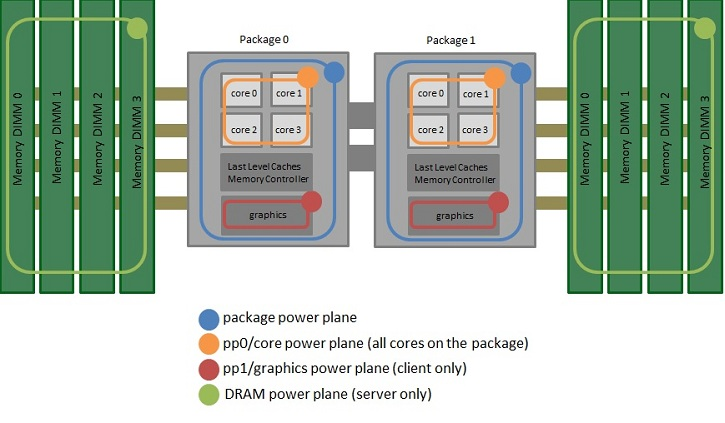
\includegraphics[width=\columnwidth]{images/power-planes-placeholder}
  \footnotesize{Source: "Intel\textsuperscript{\textregistered} Power Governor" article~\cite{dimitrov:2012}}
  \label{fig:power-planes}
\end{figure}
\end{savenotes}

With \ac{rapl}, developers can monitor energy consumption and set power limits. The access to this information is divided into different domains. Each domain is a physically meaningful domain for power management, as we can see in \figref{fig:power-planes}. The \ac{rapl} domains that are available in a platform vary across product segments. Typically, the desktop platforms have access to \{\texttt{PKG}, \texttt{PP0}, \texttt{PP1}\}, while the server platforms have access to \{\texttt{PKG}, \texttt{PP0}, \texttt{DRAM}\}. Each of these domains, provide fine-grained reports and control for power management. In \tabref{tbl:rapl-domains}, we show what each domain supports. For this work, we are interested in the \texttt{ENERGY\_STATUS} information as it provides the current measured energy consumption of a specific domain.

\begin{table}[htp]
	\centering
	\caption{List of controls supported by the RAPL domains}
	\rowcolors{1}{lightgray!30}{white}
	\begin{tabular}{ll}
	  \toprule
		\texttt{POWER\_UNIT}    & Provides the scaling factors for each unit\\
		\texttt{POWER\_LIMIT}   & Allows software to set power limits\\
		\texttt{ENERGY\_STATUS} & Reports measured actual energy usage\\
		\texttt{PERF\_STATUS}   & Reports the performance impact of power limiting\\
		\texttt{POWER\_INFO}    & Reports power range information for \ac{rapl} usage\\
	  \bottomrule
	\end{tabular}
	\label{tbl:rapl-domains}
\end{table}

The interaction with \acs{rapl} is done via \acp{msr}. Each control listed in \tabref{tbl:rapl-domains} for each domain is a separate \ac{msr}. \acp{msr} are special control registers present in the x86 instruction set that are typically used for debugging, monitoring performance, and toggling CPU features. Accessing \acp{msr} requires ring-0 access to the hardware, which is usually only allowed to the operating system kernel. This means that accessing the \ac{rapl} readings requires a kernel driver. In Linux, we do not have a specific driver to access the \ac{rapl} \acp{msr}. Instead, we have a generic \texttt{msr} driver (or kernel module) that exports \ac{msr} access to the userspace. The register readings are exposed as files inside the CPU device directories (e.g. \texttt{/dev/cpu/0/msr}). These files have read-only permission for superusers (root).

Manipulating these registers is not a very straightforward process. To do this, a developer need some knowledge of system programming and familiarity with the processor instruction set to know how to interpret the raw values exposed by the readings. Also, developers using \ac{rapl} need to handle possible register overflows. In a high power consumption scenario, for example, the \texttt{ENERGY\_STATUS} \ac{msr} of the \texttt{PKG} domain have a wraparound time of around 60 secs~\cite[p. 2465]{intel:2016}. So to abstract these low-level interfaces from Haskell developers, we present in the next sections two performance analysis tool that we extended to collect energy consumption information using \ac{rapl}.


\section{GHC Profiler}\label{sec:profiler}
A profiler is a tool for helping the development of efficient programs. Its main function is to provide the necessary information for developers to identify performance bottlenecks. So that once the hot spots in a program have been identified, the developer can work on the code to improve its performance and continuously check the effect of each modification. To achieve this goal, a profiler should keep track of important program resources. Moreover, the data gathered by the profiler must be related to the program source code in a way that is meaningful to the developer. This is usually accomplished by reporting the measurements by program structures (e.g. functions or methods) or source code structures (e.g. lines).

However, it is hard to establish this correspondence between measurements and source code for high-level languages. Usually, these languages provide abstractions and constructs that are unrelated to the way that the underlying execution engine works. Haskell is not different. Features such as polymorphism, high-order functions, and lazy evaluation make this task even harder. For example, in the presence of lazy evaluation, the evaluation of an expression can be interleaved with the evaluation of the inputs that this expression demands. This makes the resulting order of execution of expressions to bear no resemblance to the source code.

To address this problem, the \ac{ghc} profiler uses \emph{cost centres}~\cite{sansom:1995}. They are the logical components of the program to which the profiler associate the gathered data. A cost centre is simply a label to which we attribute execution costs. They are represented by annotations around expressions. So the costs incurred by the evaluation of the annotated expression are assigned to the enclosing cost centre. The cost centres can be automatically generated by the compiler or manually specified by the developer through the \texttt{\{-\# SCC \#-\}} directive. In \autoref{code:prof-mean}\footnote{This code example was extracted from \cite{sullivan:2008}}, we show an example of how it can be manually specified by the developer (line 10). In this example, all the costs incurred by the evaluation of \texttt{sum xs / fromIntegral (length xs)} will be attributed to the \texttt{mean} cost centre. It is important to point out that cost centres have a formally defined semantics~\cite{sansom:1995} that specifies how the cost attribution works.

\begin{listing}
  \caption{Haskell program to calculate the mean of a list of numbers}
  \begin{minted}{haskell}
import System.Environment
import Text.Printf

main :: IO ()
main = do
    [d] <- map read `fmap` getArgs
    printf "%f\n" (mean [1..d])

mean :: [Double] -> Double
mean xs = {-# SCC mean #-} sum xs / fromIntegral (length xs)
  \end{minted}
  \label{code:prof-mean}
\end{listing}

Currently, the \ac{ghc} profiler it is capable of measuring time and space usage. In \ac{ghc}, the profiler is part of the runtime system, which means that the profiling routines are contained within the final program executable. So to build a program for profiling, we need to pass to \ac{ghc} the \texttt{-prof} flag when compiling it. Then, to run this program in profiling mode, we need to specify it to the runtime system by passing the \texttt{+RTS -p} argument. It makes the runtime system collect time and memory usage data from the execution to produce a detailed report at the end. \figref{fig:profiler-sample} shows a profiling report for the program in \autoref{code:prof-mean}.

\begin{figure}[htp]
  \centering
  \caption{Example of profiling report for the \texttt{mean} program}
  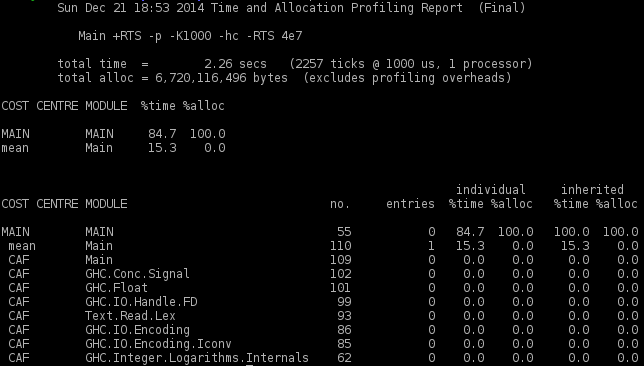
\includegraphics[width=\columnwidth]{images/profiler-placeholder}
  \footnotesize{Source: Generated by the GHC profiler}
  \label{fig:profiler-sample}
\end{figure}

As we can see in this example, we can split the report into three different sections. The first one is the header. It shows how the program was executed (which flags and arguments were passed to run it), and the total time and memory allocated during the whole execution of the program. The second part shows a break-down of the most costly cost centres. In this case, the top-level \texttt{MAIN} and the user-defined \texttt{mean}.

The third section shows a break-down by \emph{cost centre stack}~\cite{morgan:1998}. A cost centre stack is similar to a call graph. It defines a hierarchy of cost centres. In this case, we can see that \texttt{MAIN} is the root of the cost centre stack, followed by \texttt{mean} and some instances of \texttt{CAF} as children. A \ac{caf} is an expression that contains no free variables, i.e. it is a constant expression. So a \texttt{CAF} cost centre represents the one-off costs of evaluating such constants. Also, in this section of the report, we have multiple columns showing the profiling data. The time and memory usage percentage columns are shown into two different groups: \texttt{individual} and \texttt{inherited}. The former is the total of program resources spent by this cost centre while the latter is the total of program resources spent by this cost centre and its children. The other columns are \texttt{no.}, which is the id of the cost centre, and \texttt{entries}, which is the number of times that the expression enclosed by this cost centre was evaluated.

So to help on our journey of understanding the energy behavior of Haskell programs, we have extended the \ac{ghc} profiler to add a new metric: energy consumption. The idea is to collect energy consumption readings from \ac{rapl} and use the \ac{ghc} infrastructure to calculate the energy spent by each cost centre. Having this, we can display two new columns in the final report accounting the percentage of energy consumed by each cost centre. We based our solution on the approach used by the time profiler. To measure the execution time, the profiler keeps in each cost centre a tick counter. At any moment, the cost centre that is currently executing is held in a special register by the runtime system. Then, a regular clock interrupt\footnote{By default this interval is 20ms. However, the user can change it by passing a custom value to the runtime system via the \texttt{-V} argument.} runs a routine to increment this tick counter of the cost centre in execution. At the end of the program execution, the value held in the tick counter of each cost centre enables the profiler to determine and report the relative execution time cost of the different parts of the program.

Similarly, our extended version of the \ac{ghc} profiler keeps in each cost centre an accumulator. At each clock interrupt, the profiler adds to the accumulator of the cost centre that is currently in execution the energy consumed between the previous and current interrupt. This is accomplished by always saving the previous and current energy readings obtained from \ac{rapl}. If an overflow occurs on \ac{rapl} during the (extremely small) interval between two consecutive interrupts, we do not update the accumulator in this tick. At the end of the program execution, the profiler will be able to report the energy consumed by each cost centre based on its accumulator value. \figref{fig:energy-prof-report} shows the report of our extended GHC profiler the same program from \autoref{code:prof-mean}. As we can see in this report, we have now energy consumption information on each section of the report. In the header, we have the total energy consumed during the execution of the program. In the second and third sections, we have extra columns showing the percentage of energy consumed by each cost centres.

\begin{figure}[htp]
  \centering
  \caption{Example of profiling report with energy metrics for the \texttt{mean} program}
  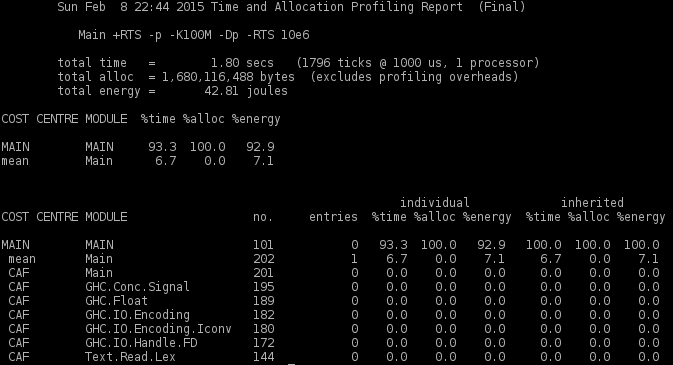
\includegraphics[width=\columnwidth]{images/energy-profiler-placeholder}
  \footnotesize{Source: Generated by the GHC profiler}
  \label{fig:energy-prof-report}
\end{figure}

Our modified version of \ac{ghc} is publicly available on GitHub\footnote{\url{http://github.com/green-haskell/ghc/tree/wip/green}}. It is based on \ac{ghc} 7.10 and includes the profiler with energy metrics. However, it is important to note that our implementation has one limitation. We can provide more accurate results only for programs that use a single capability. The main reason for this is the fact that \ac{rapl} does not provide the energy consumed by a single core. It provides only the energy consumption of the cores altogether, so if two cost centres are executing in parallel, we cannot tell how much energy each one consumed separately. However, we could easily adapt the current implementation to handle this case once the underlying \ac{api} provides the energy by core information. Also, it is easy enough to change the use of \ac{rapl} for another \ac{api} that provides energy consumption information if needed.

Despite this limitation, the profiler tool is particularly useful for providing fine-grained information about energy consumption. It enables developers to find the energy hot spots of Haskell programs. In the next section, we present another performance analysis tool called Criterion. Different from a profiler, it uses a coarse-grained approach for evaluating the performance of a program.


\section{Criterion}\label{sec:criterion}
Criterion~\cite{sullivan:2009} is a microbenchmarking library that is used to measure the performance of Haskell code. Its main objective is to estimate the cost of running a small, independent piece of code. At a first glance, it may seem that it does the same job of a profiler, but this is not the case. Criterion is not designed to finding hot spots in a program. Instead, it is useful for analyzing the cost of a given operation. A profiler is about taking a snapshot of a single execution of a program and reporting fine-grained information about its performance. Criterion, however, is about running a certain piece of code several times to analyze its performance. It reports to the developer a statistically-backed estimation of the cost of running the selected piece of code once. As Criterion does not analyze the performance for each cost centre, only the benchmarked code as a whole, we say its analysis is coarse-grained.

\begin{listing}
  \caption{Definition of a Criterion benchmark for the \texttt{fib} function}
  \begin{minted}{haskell}
import Criterion.Main

fib :: Int -> Int
fib m | m < 0     = error "negative!"
      | otherwise = go m
  where
    go 0 = 0
    go 1 = 1
    go n = go (n-1) + go (n-2)

main :: IO ()
main = defaultMain [
    bench "fib/9" (whnf fib 9)
  ]
  \end{minted}
  \label{code:fib-crit}
\end{listing}

Criterion provides a framework for both executing benchmarks as well as analyzing their results. This framework is based on a simple \ac{api} that hides most of the complexity involved in performing benchmarks. In \autoref{code:fib-crit}\footnote{This example was extracted from \url{http://www.serpentine.com/criterion/tutorial.html}}, we show an example of how to define a Criterion benchmark. Here, we want to analyze the performance of the \texttt{fib} function. The benchmark is defined to execute \texttt{fib} passing nine as argument. In this example, we are using three important functions of Criterion's \ac{api}:
\begin{itemize}
  \item \texttt{defaultMain}: takes care of executing a set of benchmarks
  \item \texttt{bench}: creates a benchmark based on an action provided by the developer
  \item \texttt{whnf}: makes sure the benchmarked action is evaluated to weak head normal form to avoid it to be evaluated only once due to Haskell's laziness
\end{itemize}

\begin{figure}[htp]
  \centering
  \caption{Output of the \texttt{fib} benchmark}
  \begin{minted}{text}
benchmarking fib/9
time                 314.4 ns   (312.2 ns .. 318.5 ns)
                     0.999 R²   (0.997 R² .. 1.000 R²)
mean                 315.3 ns   (314.0 ns .. 319.4 ns)
std dev              7.081 ns   (1.625 ns .. 14.63 ns)
variance introduced by outliers: 26% (moderately inflated)
  \end{minted}
  \footnotesize{Source: Generated by Criterion}
  \label{fig:fib-output}
\end{figure}

In \figref{fig:fib-output}, we show the output for the benchmark described in \autoref{code:fib-crit}. The first line shows \texttt{time}, which is the estimation of the time needed for executing \texttt{fib 9} once. It is obtained using an \ac{ols} regression model. Inside the parenthesis, after the time estimation, we can see the lower and upper bounds of the confidence interval that is calculated using \emph{bootstrapping}~\cite{davison:1997}. It means that when randomly resampling the data, 95\% of estimates fell between the lower and upper bounds of the interval. So the quality of the estimation is better when the bounds are closer to its value. The second line shows the coefficient of determination, or R\textsuperscript{2}, which is a statistical measure of how well the linear regression model approximates the observed measurements. An R\textsuperscript{2} between 0.99 and 1 indicates an excellent approximation. The \texttt{mean} and \texttt{std dev} lines are the mean execution time and the standard deviation, respectively. Finally, the last line indicates the degree to which the standard deviation is inflated by outlying measurements.

\begin{figure}[htp]
  \centering
  \caption{Measurement chart generated for the \texttt{fib} benchmark}
  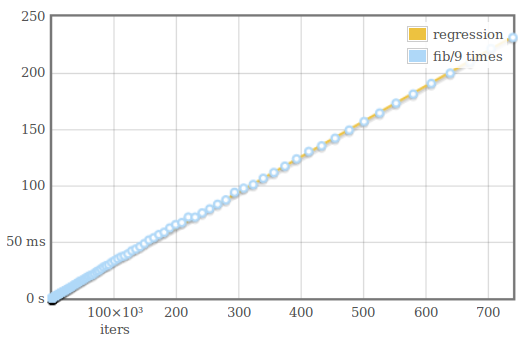
\includegraphics[width=.6\columnwidth]{images/criterion-chart} \\
  \footnotesize{Source: Generated by Criterion}
  \label{fig:crit-chart}
\end{figure}

This kind of information that Criterion provides is quite useful for making sure that the measurements are not being tainted by external factors such as other loads on the operating system. Alongside with the textual report, Criterion can also generate some charts like the one shown in \figref{fig:crit-chart}. In this graph, the $x$-axis indicates the number of loop iterations, while the $y$-axis shows the execution time for a given number of iterations. The blue circles are the raw measurements while the orange line is the linear regression generated from this data. The closer the dots are from the line; the better is the regression model.

As we can see from this example, each sample that Criterion uses for the regression model corresponds to the measurements collected during a distinct number of consecutive executions of the benchmarked code. This specific number of loop iterations is the independent variable of the regression model, which the author calls \texttt{iters}. The number of different \texttt{iters} that Criterion performs for a given benchmark depends on how much time the benchmarked code takes to run. Criterion tries to run it as much as possible so that: (1) it collects enough measurements for properly resampling the data, and (2) it generates enough measurements that have long spans of execution to outweigh the cost of measurement. For short-lived benchmarks such as \autoref{code:fib-crit}, in the order of nanoseconds, we can see that Criterion collects several samples with a high number of consecutive iterations. For longer benchmarks, in the order of tens of seconds, it is guaranteed that Criterion will collect at least five samples, from one to five iterations each, respectively\footnote{This information is not available in the library documentation. We got it by inspecting the source code.}.

\begin{figure}[htp]
  \centering
  \caption{Output with CPU cycles of the \texttt{fib} benchmark}
  \begin{minted}{text}
benchmarking fib/9
time                 317.2 ns   (314.2 ns .. 319.4 ns)
                     0.999 R²   (0.999 R² .. 1.000 R²)
mean                 314.4 ns   (313.3 ns .. 315.8 ns)
std dev              4.117 ns   (2.682 ns .. 5.398 ns)
cycles:              0.999 R²   (0.999 R² .. 1.000 R²)
  iters              1079.434   (1069.292 .. 1087.144)
  y                  924904.370 (562772.048 .. 1358678.998)
variance introduced by outliers: 13% (moderately inflated)
  \end{minted}
  \footnotesize{Source: Generated by Criterion}
  \label{fig:fib-cycle-output}
\end{figure}

Besides elapsed time, Criterion can also perform linear regression on other metrics such as CPU time, CPU cycles, bytes allocated, and the number of garbage collections. It can be done by passing the other metric as a command line argument when running the benchmark. For example, passing \texttt{-{}-regress cycles:iters} will regress the number of CPU cycles against the number of loop iterations. \figref{fig:fib-cycle-output} shows the output for such example for \autoref{code:fib-crit}. As we can see, there are three new lines in the report. The first one corresponds to the R\textsuperscript{2} for this new regression. The second line we have the estimation of how much cycles each iteration costs, which is the slope of the regression curve. The last line is where the curve intercepts the $y$-axis. This feature allows for developers to have a good overview from different perspectives about the performance of the benchmarked code.

To take advantage of Criterion in our work, we have extended it to add a new metric: energy consumption. The fact that Criterion's infrastructure already have support for estimating the cost of other metrics than elapsed time helped us to modify it in a "cleaner" way. However, the way the energy data is collected is different from the other metrics because \ac{rapl} registers are susceptible to overflows. In \autoref{code:crit-measure}, we show how Criterion currently collects the measurements. As we can see, it saves the counters before and after it executes the benchmarked code \texttt{iters} times. If we used the same approach for energy consumption, in the presence of an overflow, the data collected would be inconsistent.

\begin{listing}
  \caption{Internal function that execute the benchmarks in Criterion}
  \begin{minted}{haskell}
measure :: Benchmarkable -> Int64 -> IO (Measured, Double)
measure (Benchmarkable run) iters = do
  startStats <- getGCStats
  startTime <- getTime
  startCpuTime <- getCPUTime
  startCycles <- getCycles
  run iters
  endTime <- getTime
  endCpuTime <- getCPUTime
  endCycles <- getCycles
  endStats <- getGCStats
  let !m = applyGCStats endStats startStats $ measured {
             measTime    = max 0 (endTime - startTime)
           , measCpuTime = max 0 (endCpuTime - startCpuTime)
           , measCycles  = max 0 (fromIntegral (endCycles - startCycles))
           , measIters   = iters }
  return $ (m, endTime)
  \end{minted}
  \label{code:crit-measure}
\end{listing}

To overcome this problem, we collect the energy consumption slightly different from the other metrics. We have to read the \ac{rapl} counters constantly during the benchmark execution in order to detect overflows. One way we could accomplish this task is by spawning a background thread to collect the energy data. However, this approach is not very lightweight. It would increase the measurement overhead and possibly influence the result of more sensitive benchmarks. So instead, we have used native Linux signals. So it works as following: before Criterion runs the benchmarked code, we register a Linux signal to be fired every 10ms. When registering this signal, we attach a signal handler that we implemented. Inside this handler, we read the \ac{rapl} counters, check if an overflow happened, and if not, we save the energy consumed between the last two readings into an internal accumulator. At the end, when the benchmark finishes executing, we can deregister the signal and get the value held by the accumulator, which is the energy measurements.

To implement this solution, similarly to how the time and cycles data is collected, we use native C code. The communication with the Criterion code, which is implemented in Haskell, is done straightforwardly via foreign function interface (FFI) calls. The interface with Linux to use signals is done using the \texttt{sigaction} and \texttt{setitimer} syscalls. The source code of our modified version of Criterion is publicly available on GitHub\footnote{\url{http://github.com/green-haskell/criterion}}. In \figref{fig:fib-energy-output}, we show an example of a benchmarks output using Criterion with the energy metrics. In this case, the benchmark was executed passing the \texttt{-{}-regress energy:iters} argument to regress energy consumption against the number of loop iterations. As we can see in the output, a single execution of this program is expected to consume 180.9 joules of energy.

\begin{figure}[htp]
  \centering
  \caption{Output example of Criterion with energy metrics}
	\begin{minted}{text}
benchmarking dining-philosophers (forkOS | MVar)
time                 2.183 s    (1.915 s .. 2.510 s)
                     0.997 R²   (0.991 R² .. 1.000 R²)
mean                 2.179 s    (2.113 s .. 2.212 s)
std dev              57.17 ms   (0.0 s .. 57.19 ms)
energy:              0.999 R²   (0.997 R² .. 1.000 R²)
  iters              180.947    (164.629 .. 200.826)
  y                  0.937      (-71.359 .. 37.230)
variance introduced by outliers: 19% (moderately inflated)
  \end{minted}
  \footnotesize{Source: Generated by Criterion}
  \label{fig:fib-energy-output}
\end{figure}

Criterion is a powerful tool. It provides a robust methodology for performing benchmarks of Haskell code. In the next chapter, we present an empirical study where Criterion was heavily employed to measure the performance and energy consumption of various concurrent programming constructs.
